% 图 24.5 —— 由 `checks/emit_hand.py` 自动拼出（probe 精测 + prims2 图元分解）
%%
% ⚠ 这是**稿子不是成品**：跑 `checks/checkhand.py 24.5` 看指标 + 看叠合图。
%%
%% ⚠ 待核：
%   · 本图 probe 报出阴影族 1 个 —— **本脚本不生成阴影**（要照原书手写）；prims2 的 strokes 里可能含阴影线，核对时留意别画重
%   · 可疑字形 1 项（空心圈 ⊙ 常被认成字母 o）—— 见文件末
%%
\documentclass[12pt]{standalone}
\usepackage{fontspec}
\setsansfont{Arial}
\newfontfamily\mfallback{DejaVu Sans}
\usepackage{tikz}
\begin{document}
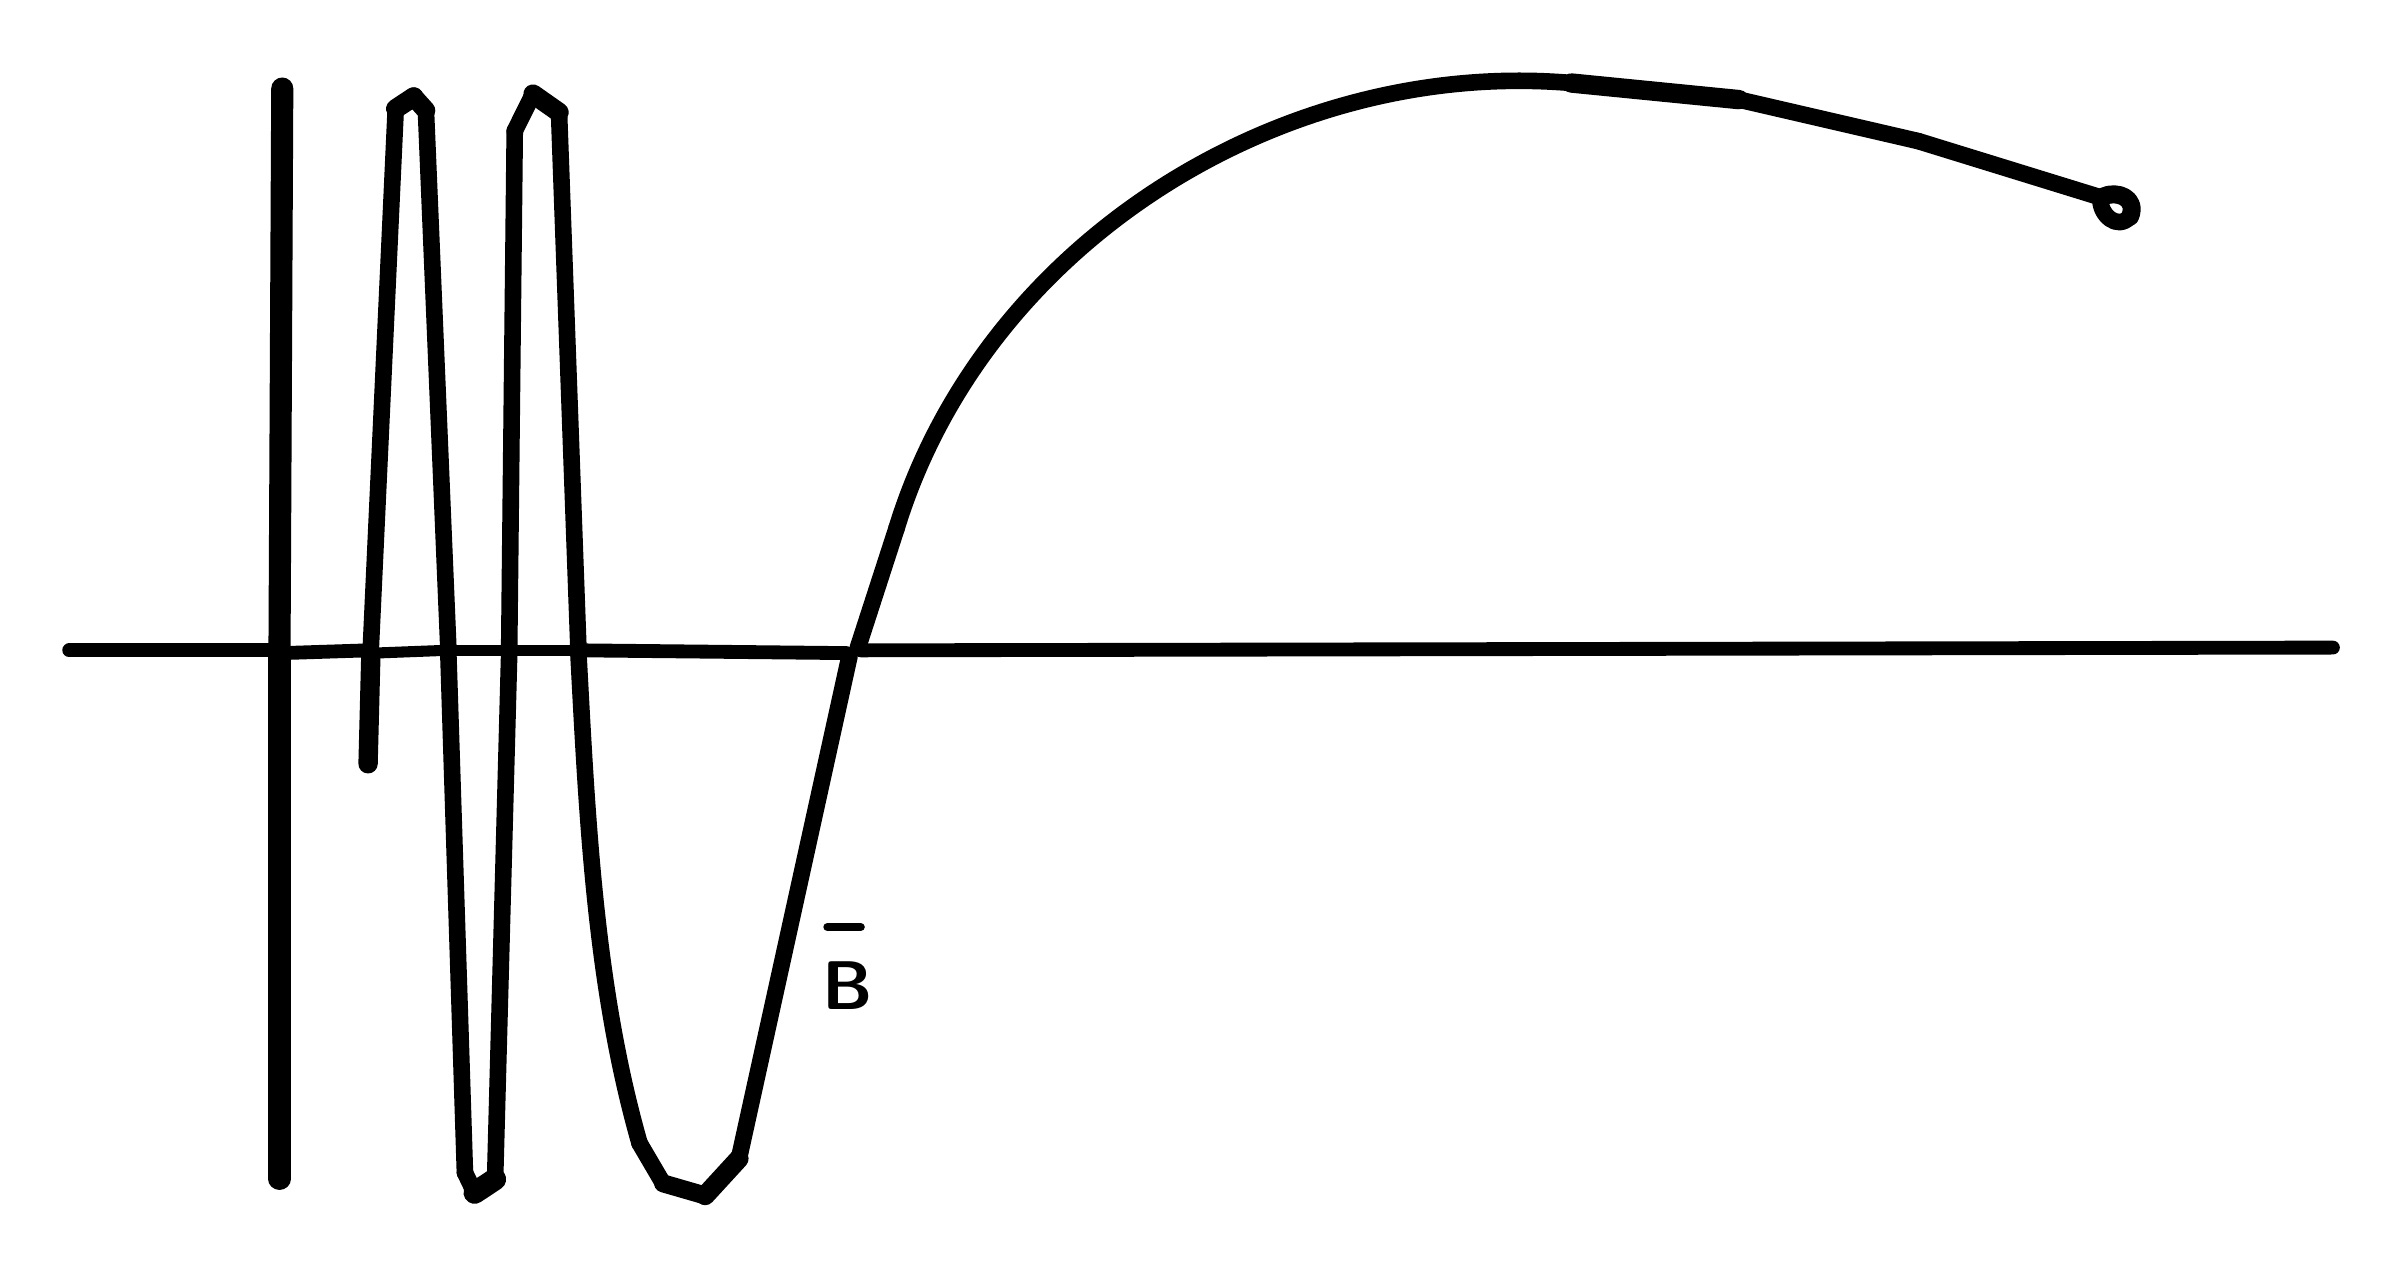
\begin{tikzpicture}[x=1pt, y=-1pt, line width=5.0pt, line cap=round, line join=round]

  %% ════ 直线段（prims2 的 strokes）════
  \draw[line width=5.0pt] (200.0,225.0) -- (296.0,226.0);
  \draw[line width=5.0pt] (833.0,224.0) -- (301.0,225.0);
  \draw[line width=6.0pt] (174.0,224.0) -- (176.0,37.3);
  \draw[line width=6.0pt] (176.0,37.3) -- (182.6,24.0);
  \draw[line width=7.0pt] (182.6,24.0) -- (192.0,30.6);
  \draw[line width=6.0pt] (192.0,30.6) -- (199.0,224.0);
  \draw[line width=5.0pt] (90.0,225.0) -- (15.0,225.0);
  \draw[line width=6.0pt] (174.0,226.0) -- (168.9,416.1);
  \draw[line width=8.0pt] (168.9,416.1) -- (161.5,421.0);
  \draw[line width=6.0pt] (161.5,421.0) -- (158.0,413.7);
  \draw[line width=6.0pt] (158.0,413.7) -- (152.0,226.0);
  \draw[line width=4.0pt] (151.0,225.0) -- (125.0,226.0);
  \draw[line width=4.0pt] (175.0,225.0) -- (198.0,225.0);
  \draw[line width=6.0pt] (152.0,224.0) -- (143.9,29.9);
  \draw[line width=6.8pt] (143.9,29.9) -- (139.5,25.0);
  \draw[line width=7.0pt] (139.5,25.0) -- (133.0,29.3);
  \draw[line width=6.0pt] (133.0,29.3) -- (124.0,224.0);
  \draw[line width=8.0pt] (91.0,224.0) -- (92.0,22.0);
  \draw[line width=5.0pt] (123.0,225.0) -- (92.0,226.0);
  \draw[line width=6.0pt] (297.0,227.0) -- (257.0,408.7);
  \draw[line width=7.0pt] (257.0,408.7) -- (244.8,422.0);
  \draw[line width=6.5pt] (244.8,422.0) -- (229.6,417.6);
  \draw[line width=6.0pt] (229.6,417.6) -- (221.1,403.1);
  \draw[line width=3.0pt] (289.0,325.0) -- (301.0,325.0);
  \draw[line width=4.0pt] (153.0,225.0) -- (173.0,225.0);
  \draw[line width=7.0pt] (123.0,266.0) -- (124.0,227.0);
  \draw[line width=6.0pt] (300.0,224.0) -- (314.0,180.8);
  \draw[line width=7.0pt] (557.8,20.0) -- (618.4,26.0);
  \draw[line width=6.0pt] (618.4,26.0) -- (683.2,41.0);
  \draw[line width=6.0pt] (683.2,41.0) -- (748.0,61.0);
  \draw[line width=8.0pt] (91.0,227.0) -- (91.0,416.0);

  %% ════ 曲线（prims2 的 curves —— 三段式，坐标同为 (y,x)）════
  \draw[line width=6.0pt] (749.0,62.0) .. controls (748.7,67.3) and (754.9,73.5) .. (759.7,68.3);
  \draw[line width=6.5pt] (759.7,68.3) .. controls (762.4,61.5) and (755.0,58.7) .. (750.0,61.0);
  \draw[line width=6.0pt] (221.1,403.1) .. controls (205.0,346.8) and (202.2,286.3) .. (199.0,226.0);
  \draw[line width=6.0pt] (314.0,180.8) .. controls (345.4,78.5) and (452.3,11.0) .. (557.8,20.0);

  %% ════ 标签（probe 直接给的 \node 行）════
  %% ⚠ 全部补了 fill=white：文字在最上层，否则与曲线交叉干扰
     \node[anchor=center,inner sep=0pt,fill=white,font=\fontsize{30.2}{37.8}\selectfont] at (296.3,346.0) {\textsf{\textbf{\textit{B}}}};   % box(285,334,19,23)

  % 钉死画布：否则超出的图元/控制点会把页面撑大，1:1 回比就失准
  \pgfresetboundingbox
  \path[use as bounding box] (0,0) rectangle (844,436);
\end{tikzpicture}
\end{document}

% ⚠ 待核清单（probe 拿不准，人眼过一遍）：
%   · 未识别/跳过：⑤ 跳过/未识别的字形
